\documentclass[border=6pt]{standalone}
\usepackage{amsmath,amssymb}
\usepackage{tikz}
\usetikzlibrary{decorations.pathreplacing,calc,positioning}
% TikZ styles and helpers shared by figures/circuits.tex and figures/circuits_qsvt.tex
\tikzset{
  wire/.style={line width=0.55pt},
  gate/.style={draw,fill=white,minimum height=6.2mm,minimum width=7.5mm,inner sep=1.5pt,font=\small,line width=0.55pt},
  wgate/.style={gate,minimum width=13mm},
  ctrl/.style={circle,fill=black,inner sep=0pt,minimum size=1.9mm},
  octrl/.style={circle,draw,fill=white,inner sep=0pt,minimum size=1.9mm,line width=0.55pt},
  targ/.style={circle,draw,inner sep=0pt,minimum size=3.2mm,line width=0.55pt},
  meter/.style={draw,fill=white,minimum height=6.2mm,minimum width=7.5mm,line width=0.55pt},
  reg/.style={font=\small,anchor=east},
  blk/.style={font=\footnotesize,anchor=north,text=black!65},
  st/.style={font=\footnotesize,anchor=south,text=blue!45!black},
  brace/.style={decorate,decoration={brace,mirror,amplitude=2.2pt},line width=0.4pt,black!60},
  slash/.style={},
}
\newcommand{\slashwire}[3]{% x y label : the /n mark on a multi-qubit wire
  \draw[line width=0.7pt] (#1cm-1.3mm,#2cm-1.6mm) -- (#1cm+1.3mm,#2cm+1.6mm);
  \node[font=\scriptsize,anchor=south west,inner sep=0.4pt] at (#1cm+0.9mm,#2cm+0.9mm) {#3};}
\newcommand{\vsep}[3]{% x ybot ytop : a dashed block boundary
  \draw[dashed,black!45,line width=0.4pt] (#1cm,#2cm) -- (#1cm,#3cm);}


% box spanning wires: x, ytop, ybot, width(cm), label
\newcommand{\mb}[5]{\draw[fill=white,line width=0.55pt] (#1-#4/2,#2+0.31) rectangle (#1+#4/2,#3-0.31); \node[font=\small] at (#1,{(#2+#3)/2}) {#5};}
\newcommand{\gt}[3]{\node[gate] at (#1,#2) {#3};}
\newcommand{\wg}[4]{\node[gate,minimum width=#3] at (#1,#2) {#4};}
\newcommand{\ct}[2]{\node[ctrl] at (#1,#2) {};}
\newcommand{\oc}[2]{\node[octrl] at (#1,#2) {};}
\newcommand{\vl}[3]{\draw[wire] (#1,#2) -- (#1,#3);}
\newcommand{\tg}[2]{\node[targ] at (#1,#2) {}; \draw[wire] (#1,#2-0.16) -- (#1,#2+0.16);}
\newcommand{\meas}[2]{\node[meter] at (#1,#2) {}; \draw[wire] (#1-0.25,#2-0.12) arc (160:20:0.27); \draw[wire,-latex] (#1,#2-0.12) -- (#1+0.2,#2+0.12);}
\newcommand{\wires}[3]{\foreach \y in {#3} {\draw[wire] (#1,\y) -- (#2,\y);}}
\newcommand{\lab}[3]{\node[reg] at (#1,#2) {#3};}
\definecolor{hitp}{RGB}{118,68,160}
\definecolor{classic}{RGB}{90,90,90}
\newcommand{\cbox}[6]{\draw[rounded corners=3pt,fill=black!4,draw=black!45,line width=0.5pt] (#1,#2) rectangle (#3,#4); \node[font=\footnotesize,align=center,text width=#6] at ({(#1+#3)/2},{(#2+#4)/2}) {#5};}
\begin{document}

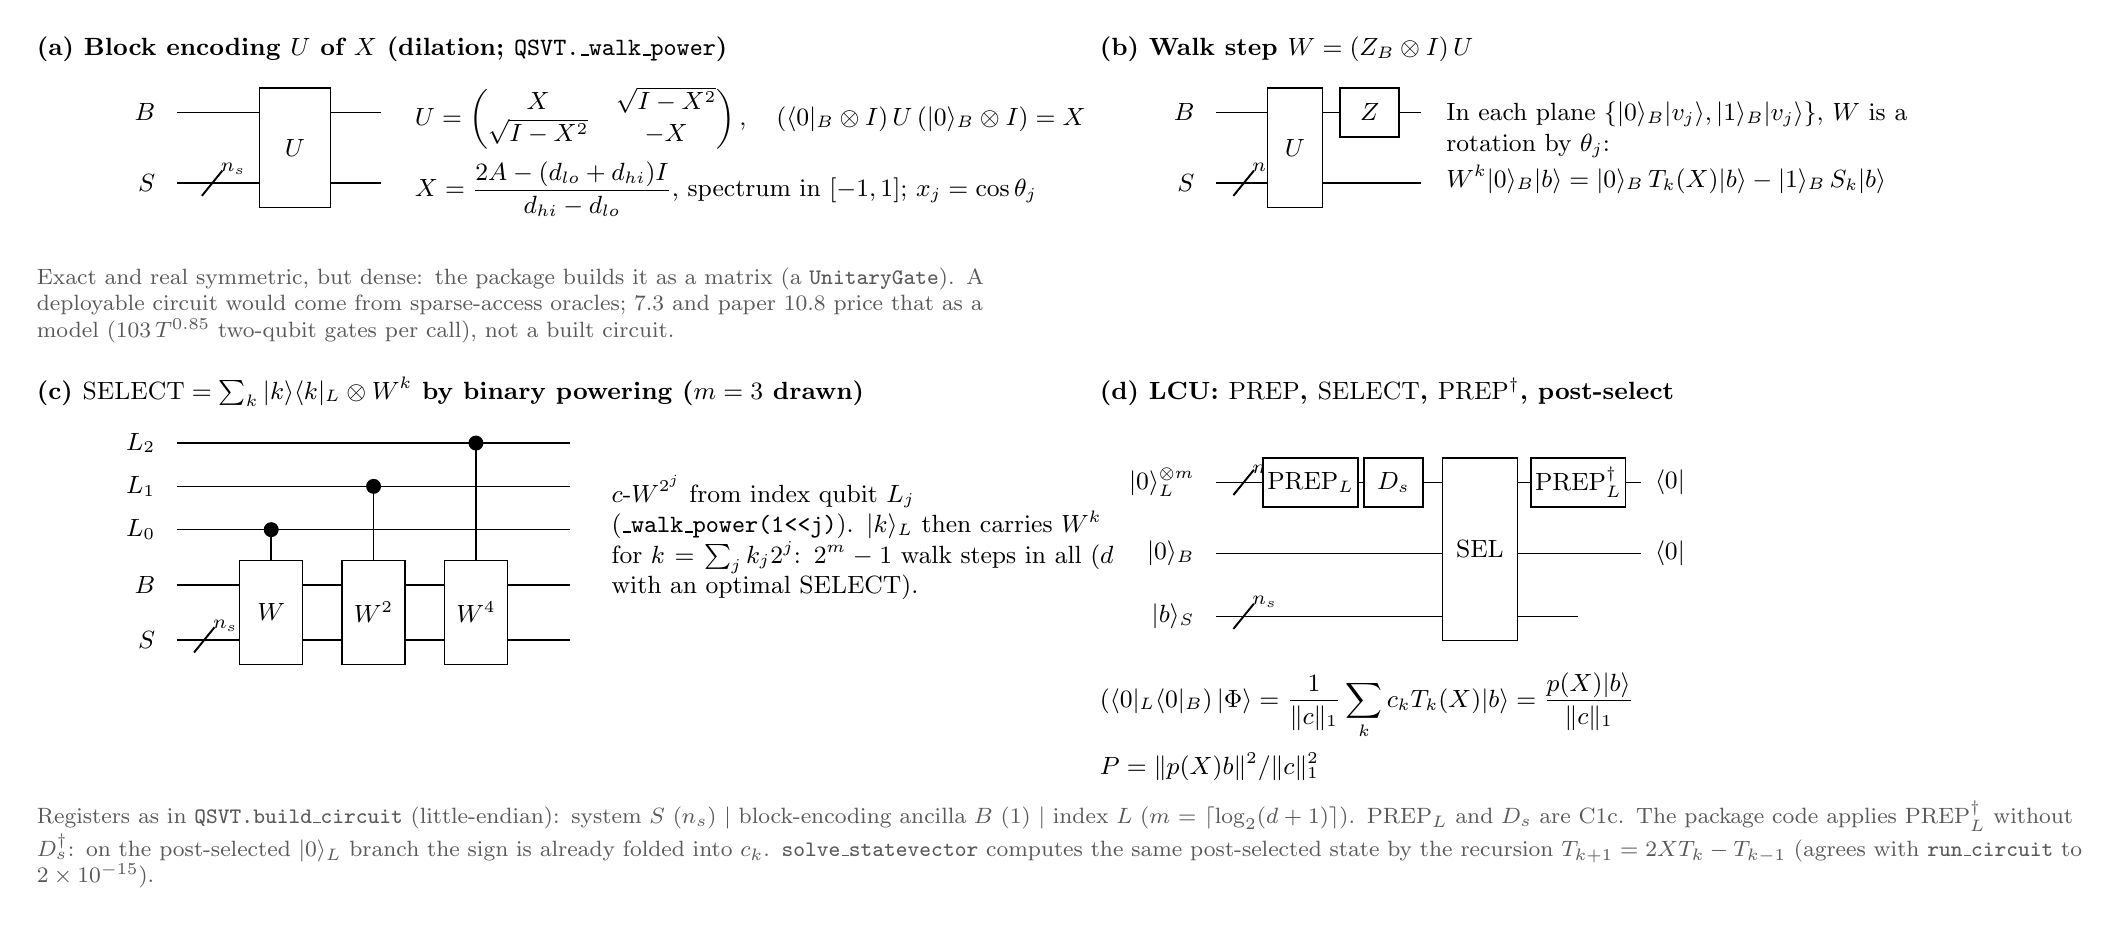
\begin{tikzpicture}[x=1cm,y=1cm]
% (a) block encoding
\node[anchor=west,font=\small\bfseries] at (-1.9,1.2) {(a) Block encoding $U$ of $X$ (dilation; \texttt{QSVT.\_walk\_power})};
\lab{-0.15}{0.4}{$B$} \lab{-0.15}{-0.5}{$S$}
\wires{0}{2.6}{0.4,-0.5} \slashwire{0.45}{-0.5}{$n_s$}
\mb{1.5}{0.4}{-0.5}{0.9}{$U$}
\node[font=\small,anchor=west,text width=8.6cm] at (2.9,-0.1) {$U=\begin{pmatrix}X&\sqrt{I-X^2}\\ \sqrt{I-X^2}&-X\end{pmatrix},\quad (\langle0|_B\otimes I)\,U\,(|0\rangle_B\otimes I)=X$\\[3pt] $X=\dfrac{2A-(d_{lo}+d_{hi})I}{d_{hi}-d_{lo}}$, spectrum in $[-1,1]$; $x_j=\cos\theta_j$};
\node[font=\footnotesize,anchor=west,text=black!65,text width=12.5cm] at (-1.9,-2.05) {Exact and real symmetric, but dense: the package builds it as a matrix (a \texttt{UnitaryGate}). A deployable circuit would come from sparse-access oracles; 7.3 and paper 10.8 price that as a model ($103\,T^{0.85}$ two-qubit gates per call), not a built circuit.};
% (b) walk
\begin{scope}[shift={(13.2,0)}]
\node[anchor=west,font=\small\bfseries] at (-1.6,1.2) {(b) Walk step $W=(Z_B\otimes I)\,U$};
\lab{-0.15}{0.4}{$B$} \lab{-0.15}{-0.5}{$S$}
\wires{0}{2.6}{0.4,-0.5} \slashwire{0.35}{-0.5}{$n_s$}
\mb{1.0}{0.4}{-0.5}{0.7}{$U$} \gt{1.95}{0.4}{$Z$}
\node[font=\small,anchor=west,text width=6.2cm] at (2.8,-0.05) {In each plane $\{|0\rangle_B|v_j\rangle,|1\rangle_B|v_j\rangle\}$, $W$ is a rotation by $\theta_j$:\\[2pt] $W^k|0\rangle_B|b\rangle=|0\rangle_B\,T_k(X)|b\rangle-|1\rangle_B\,S_k|b\rangle$};
\end{scope}
% (c) SELECT
\begin{scope}[shift={(0,-4.9)}]
\node[anchor=west,font=\small\bfseries] at (-1.9,1.75) {(c) $\mathrm{SELECT}=\sum_k|k\rangle\langle k|_L\otimes W^k$ by binary powering ($m=3$ drawn)};
\lab{-0.15}{1.1}{$L_2$} \lab{-0.15}{0.55}{$L_1$} \lab{-0.15}{0}{$L_0$} \lab{-0.15}{-0.7}{$B$} \lab{-0.15}{-1.4}{$S$}
\wires{0}{5.0}{1.1,0.55,0,-0.7,-1.4} \slashwire{0.35}{-1.4}{$n_s$}
\ct{1.2}{0} \vl{1.2}{0}{-1.1} \mb{1.2}{-0.7}{-1.4}{0.8}{$W$}
\ct{2.5}{0.55} \vl{2.5}{0.55}{-1.1} \mb{2.5}{-0.7}{-1.4}{0.8}{$W^2$}
\ct{3.8}{1.1} \vl{3.8}{1.1}{-1.1} \mb{3.8}{-0.7}{-1.4}{0.8}{$W^4$}
\node[font=\small,anchor=west,text width=6.6cm,align=left] at (5.4,-0.1) {$c\text{-}W^{2^j}$ from index qubit $L_j$ (\texttt{\_walk\_power(1<<j)}). $|k\rangle_L$ then carries $W^k$ for $k=\sum_jk_j2^j$: $2^m-1$ walk steps in all ($d$ with an optimal SELECT).};
\end{scope}
% (d) LCU sandwich
\begin{scope}[shift={(13.2,-4.9)}]
\node[anchor=west,font=\small\bfseries] at (-1.6,1.75) {(d) LCU: $\mathrm{PREP}$, $\mathrm{SELECT}$, $\mathrm{PREP}^\dagger$, post-select};
\lab{-0.15}{0.6}{$|0\rangle_L^{\otimes m}$} \lab{-0.15}{-0.3}{$|0\rangle_B$} \lab{-0.15}{-1.1}{$|b\rangle_S$}
\wires{0}{5.4}{0.6,-0.3} \wires{0}{4.6}{-1.1} \slashwire{0.35}{0.6}{$m$} \slashwire{0.35}{-1.1}{$n_s$}
\wg{1.2}{0.6}{11mm}{$\mathrm{PREP}_L$} \gt{2.25}{0.6}{$D_s$}
\mb{3.35}{0.6}{-1.1}{0.95}{\small SEL}
\wg{4.6}{0.6}{11mm}{$\mathrm{PREP}_L^\dagger$}
\node[font=\small,anchor=west] at (5.45,0.6) {$\langle0|$}; \node[font=\small,anchor=west] at (5.45,-0.3) {$\langle0|$};
\node[font=\small,anchor=west,text width=9cm] at (-1.6,-2.5) {$(\langle0|_L\langle0|_B)\,|\Phi\rangle=\dfrac{1}{\lVert c\rVert_1}\displaystyle\sum_kc_kT_k(X)|b\rangle=\dfrac{p(X)|b\rangle}{\lVert c\rVert_1}$\\[4pt] $P=\lVert p(X)b\rVert^2/\lVert c\rVert_1^2$};
\end{scope}
\node[font=\footnotesize,anchor=west,text=black!65,text width=26cm] at (-1.9,-8.9) {Registers as in \texttt{QSVT.build\_circuit} (little-endian): system $S$ ($n_s$) \textbar\ block-encoding ancilla $B$ (1) \textbar\ index $L$ ($m=\lceil\log_2(d+1)\rceil$). $\mathrm{PREP}_L$ and $D_s$ are C1c. The package code applies $\mathrm{PREP}_L^\dagger$ without $D_s^\dagger$: on the post-selected $|0\rangle_L$ branch the sign is already folded into $c_k$. \texttt{solve\_statevector} computes the same post-selected state by the recursion $T_{k+1}=2XT_k-T_{k-1}$ (agrees with \texttt{run\_circuit} to $2\times10^{-15}$).};
\end{tikzpicture}
\end{document}
